\chapterimage{unidades/1_computadoras/1_computadoras/imagenes/cover}
\chapterimagedescription{Placa base de una computadora con sus circuitos impresos}
\chapterimageauthor{Fotografía de Blickpixel}

\chapter{Computadoras}
\index{Computadora}
\label{chap:computadoras}

Las utilizamos todos los días, rigen nuestra vida cotidiana, y el mundo moderno
dejaría de funcionar sin ellas. Las computadoras son omnipresentes en nuestro
día a día, ya sea que trabajemos directamente con ellas o no. Pero, ¿Qué es
exactamente una computadora?, y más aún ¿Pará que sirve?.

Este capítulo intenta responder todas esas interrogantes y generar un glosario
de los términos más comunes en informática. No es el fin de este capítulo
centrarnos en detalles, sino obtener un panorama general de una computadora y
como esta funciona. Capítulos siguientes retomarán este contenido y
complementarán aportando detalles más específicos.

Comencemos entonces por definir qué es una computadora:

\begin{definition}
    Una \textbf{computadora} es una máquina electrónica o electromecánica que
    recibe datos, los analiza, procesa y transforma, convirtiéndolos en
    información conveniente y útil para el posterior uso por seres
    humanos.\autocite[vid. p.10]{gookin_2005}
\end{definition}

\wraplimage[0.25]{unidades/1_computadoras/1_computadoras/imagenes/apple_II.jpg}
{Vieja Apple II.} {Exhibición del Musée Bolo, Lausana, Suiza.}

Es decir, una computadora es un dispositivo cuya única función es la de procesar
datos. Esos datos, también suelen ser llamados ``información'', y podrían ser
procesados por un ser humano sin ningún problema. Lo que hace a una computadora
realmente interesante es que \textbf{es capaz de procesar gran cantidad de datos
en muy poco tiempo}. Así, una tarea que implique procesar grandes volúmenes de
información, o procesarla de formas complejas (tarea que le podría llevar a una
persona meses, o incluso años) a una computadora le puede llevar pocos
segundos.\autocite[vid. p.8]{clark_scott_2009}

Toda computadora está formada físicamente por numerosos componentes electrónicos
y electro-mecánicos. Además, toda computadora cuenta con algún dispositivo que
permite ingresar datos a la misma (por ejemplo, un teclado o un mouse), y algún
otro dispositivo que permite ver los datos que la computadora procesó (por
ejemplo, un monitor o una impresora).

Cuando se habla de computadora, generalmente pensamos en la típica
\textbf{computadora de escritorio} (con su voluminoso gabinete, un monitor,
teclado y mouse). Sin embargo, las computadoras tienen hoy en día formas cada
vez más diversas, como por ejemplo, las \textbf{notebooks}, y sus primas
pequeñas las \textbf{netbooks}. Las \textbf{tablets}, los \textbf{celulares} e
incluso los \textbf{relojes inteligentes} son también ejemplos de computadoras.
Cada una tiene sus particularidades, por ejemplo, la forma de ingresar datos en
una notebook no es la misma que en un celular. Sin embargo, todas son
computadoras y comparten características comunes.

De hecho, la definición de computadora que utilizamos es tan amplia, que abarca
una serie de dispositivos que en general no clasificaríamos como computadoras,
pero que, por sus características, lo son. Además de las anteriormente
mencionadas podríamos incluir también:

\begin{itemize}
    \item \textbf{Consolas de videojuegos}
    \item \textbf{Juguetes electrónicos}
    \item \textbf{Sistemas de domótica (IoT)}
    \item \textbf{Computadoras de abordo (en autos, barcos y aviones)}
    \item \textbf{Robots}
    \item \textbf{Calculadoras graficadoras programables}
    \item \textbf{Microcontroladores}
\end{itemize}

Muchos otros dispositivos también podrían ser consideradas computadoras, o
incluyen computadoras como un componente fundamental para poder funcionar.
\autocite[introduction]{ceruzzi_2003}

\begin{knowwhat}[En realidad]
Técnicamente cualquier dispositivo electrónico que realice cálculos (cómputos)
es una computadora. Sin embargo, en general nos referimos como computadora a
aquellos dispositivos que son ``programables'', es decir, que pueden
configurarse para llevar a cabo distintas tareas por parte del usuario. Está
distinción no nos resulta relevante.
\end{knowwhat}

Una computadora está constituida por dos partes fundamentales: El
\textbf{hardware}, que comprende a la \textbf{parte física} de una computadora,
y el \textbf{software}, es decir, la parte \textbf{parte lógica}. A continuación
trataremos más en detalle ambas partes.

\section{Hardware (parte física)}
\index{Hardware}
\index{Parte Fisica@Parte Física}
\label{chap:computadoras:sec:hardware}

Comencemos por definir a qué nos referimos cuando hablamos de hardware:

\begin{definition}
    El \textbf{hardware} comprende todos los elementos físicos que componen a la
    computadora. Es decir, el conjunto de circuitos, cables, perillas, palancas,
    botones, luces, displays, dispositivos de impresión, motores, imanes, placas
    metálicas, etc.\autocite[vid. p.12]{gookin_2005}
\end{definition}

Una definición más pragmática sería: \textbf{si no funciona y lo puedo patear,
es hardware}.

Los componentes físicos que tenga la computadora, serán dependientes del tipo de
computadora con la que contemos. Así por ejemplo, algunas tendrán un teclado,
mientras que otras contarán con una pantalla táctil; unas tendrán un monitor,
mientras otras tendrán un display indicador; etc.

Muchos de estos dispositivos trabajan con elementos que no son puramente
eléctricos, sino físicos o mecánicos. A estos se los denomina
\textbf{dispositivos analógicos}. En general, los datos que emiten o reciben
tienen forma de onda (son valores continuos sobre un rango).

Los dispositivos que no emplean partes mecánicas, sino solamente electrónicas,
suelen emitir o recibir datos discretos (valores puntuales, que no conforman un
espectro). Este tipo de dispositivos se denominan \textbf{dispositivos
digitales}.

La mayoría de las computadoras de hoy en días (aunque no siempre es así, ni
tampoco fue así siempre) contienen una serie de partes relativamente estándar
entre las que destacan:
\begin{description}
    \item[Fuente de alimentación (Fuente de poder)]\index{Fuente de
        Alimentacion@Fuente de Alimentación} Se trata de un transformador de
        electricidad que modifica la corriente que le llega (por ejemplo, desde
        un enchufe en la pared, con 220V, o desde una batería de litio), al
        voltaje que requiere la máquina para funcionar (por ejemplo, 12V, 5V,
        etc.). Como las computadoras son aparatos electrónicos, todas requieren
        electricidad de alguna forma. Este dispositivo se encarga entonces de
        darle energía a todos los otros componentes de la máquina.
    \item[Motherboard (Placa base o tarjeta madre)]\index{Motherboard} Consiste
        en una tarjeta o placa, que contiene los circuitos principales de la
        computadora impresos en un material conductivo (cobre, oro, etc.) sobre
        su superficie. La placa cuenta con ranuras (la mayoría estandarizadas)
        en donde se conectan los diversos componentes del equipo (aunque a veces
        los mismos pueden estar soldados directamente a la placa). Sus circuitos
        se encargan de conectar y a los diversos componentes entre sí,
        permitiendo que la electricidad fluya de uno a otro componente.
    \item[CPU (Central Processing Unit o Procesador)]\index{CPU} Es lo que se
        conoce como un circuito integrado. Está compuesto de millones de
        transistores microscópicos, que son capaces de realizar miles de
        millones de cálculos por segundo. Además el CPU se encarga de coordinar
        al resto de los componentes, manejar los datos que entran, los que salen
        etc.
    \item[Memoria RAM]\index{Memoria RAM} Otro importante circuito integrado,
        pero que no realiza cálculos, sino que almacena información. Es el lugar
        donde el equipo almacena los datos temporales de las cuentas y acciones
        que va realizando (no debe confundirse con el lugar en donde se guardan
        datos a largo plazo). La memoria RAM solamente almacena información
        mientras la computadora esté encendida. Una vez la máquina se apaga, la
        información se pierde.
\end{description}

Estos componentes son lo que en general llamamos \textbf{computadora} en sí
misma. El resto de los componentes son conocidos como periféricos. Los
periféricos se conectan a la \textbf{computadora} para agregar capacidades de
entrada y salida de información.\autocite[cap. 2]{gookin_2006}

En el lenguaje coloquial, usamos el término \textbf{computadora} para referirnos
tanto a los componentes principales como a todos los periféricos conectados a
los mismos. En general utilizamos el término con esta última acepción pero al
hablar de periféricos el término computadora suele referir solo a los
componentes principales.

\subsection{Periféricos}
\index{Perifericos@Periféricos}
\label{chap:computadoras:subsec:perifericos}

Los \textbf{periféricos} son componentes de hardware adicionales que se acoplan
a los componentes principales de la computadora. El nombre deriva de que los
mismos se colocan en torno a estos (en la periferia).

\begin{definition}\index{Periferico@Periférico} Un \textbf{periférico} es un
    dispositivo de hardware que se acopla a los componentes centrales de una
    computadora y que permiten el ingreso y/o egreso de información a la
    misma.\autocite[vid. p. 363]{laplante_2000}
\end{definition}

\image{unidades/1_computadoras/1_computadoras/imagenes/hardware.jpg}
{Diversos componentes de hardware de una computadora de escritorio.}
{Ilustración de GregoryJCL.}

Los periféricos solo tienen por finalidad el permitir ingresar datos o
información a los componentes principales de la computador, o por el contrario,
extraer la información que los componentes principales hayan generado para
presentársela al usuario. Algunos de estos dispositivos cumplen ambas funciones.
El almacenamiento a largo plazo de información también puede considerarse como
entrada y salida de datos, y por eso los dispositivos que almacenan información
son considerados también periféricos.

Los periféricos se \textbf{clasifican en 4 categorías}, según si permiten
ingresar datos, extraerlos, ingresarlos y extraerlos al mismo tiempo, o
almacenar los datos a largo plazo.

\subsubsection*{Periféricos de Entrada}
\index{Perifericos de Entrada@Periféricos de Entrada}
\label{chap:computadoras:subsubsec:perifericos_entrada}

Los periféricos de entrada son aquellos que utilizamos para ingresar datos a la
computadora. El dispositivo lee lo que el usuario ingresa de forma analógica
(por ejemplo, que palancas accionó, o que botones presionó) y traduce esa
información a impulsos eléctricos que serán enviados a la computadora para que
esta procese la información ingresada.\autocite[p. 246]{laplante_2000}

Ejemplos comunes de este tipo de periféricos son:

\begin{minipage}{0.45\textwidth}
    \begin{itemize}
        \item \textbf{Teclado}
        \item \textbf{Mouse}
        \item \textbf{Trackpad}
        \item \textbf{Micrófonos}
    \end{itemize}
\end{minipage}
\begin{minipage}{0.45\textwidth}
    \begin{itemize}
        \item \textbf{Cámaras Digitales}
        \item \textbf{Webcams}
        \item \textbf{Joysticks}
        \item \textbf{Scanners}
    \end{itemize}
\end{minipage}

Fuera de los tradicionales, hoy en día los dispositivos móviles cuentan con una
amplia cantidad de periféricos de entrada en forma de sensores. Además,
computadoras que comprenden sistemas más específicos, como de automatización
industrial, pueden contar con sensores más especializados aún. Algunos ejemplos
incluyen:

\begin{minipage}{0.45\textwidth}
    \begin{itemize}
        \item \textbf{Giroscopios}
        \item \textbf{Potenciómetros}
        \item \textbf{GPS}
        \item \textbf{Sensores de luz}
        \item \textbf{Sensores de temperatura}
        \item \textbf{Detectores de humo/$CO_2$}
    \end{itemize}
\end{minipage}
\begin{minipage}{0.45\textwidth}
    \begin{itemize}
        \item \textbf{Perillas, palancas y botones}
        \item \textbf{Sensores de movimiento}
        \item \textbf{Sensores de humedad}
        \item \textbf{Lectores de tarjetas magnéticas}
        \item \textbf{Lectores RFID}
        \item \textbf{Lectores de tarjetas perforadas}
    \end{itemize}
\end{minipage}

La gran mayoría de los periféricos de entrada suelen ser sensores analógicos
cuya señal es transformada en digital por algún componente para ser luego
enviada al CPU. También existen por supuesto casos de periféricos completamente
digitales.

\subsubsection*{Periféricos de Salida}
\index{Perifericos de Salida@Periféricos de Salida}
\label{chap:computadoras:subsubsec:perifericos_salida}

Los dispositivos de salida incluyen todos aquellos dispositivos mediante los
cuales la computadora nos muestra indicaciones de los datos que procesó, o que
se encuentra procesando.\autocite[p. 352]{laplante_2000} Algunos ejemplos de
estos dispositivos incluyen:

\begin{minipage}{0.45\textwidth}
    \begin{itemize}
        \item \textbf{Pantallas o monitores}
        \item \textbf{Impresoras}
        \item \textbf{Displays digitales}
    \end{itemize}
\end{minipage}
\begin{minipage}{0.45\textwidth}
    \begin{itemize}
        \item \textbf{Luces (LEDs)}
        \item \textbf{Parlantes}
        \item \textbf{Auriculares}
    \end{itemize}
\end{minipage}

Nuevamente podemos encontrar sistemas con casos más específicos, como puede ser:

\begin{minipage}{0.45\textwidth}
    \begin{itemize}
        \item \textbf{Proyectores}
        \item \textbf{Dispositivos de lectura braille}
        \item \textbf{Fax}
    \end{itemize}
\end{minipage}
\begin{minipage}{0.45\textwidth}
    \begin{itemize}
        \item \textbf{Plotter}
        \item \textbf{Motores}
        \item \textbf{Impresoras 3D}
    \end{itemize}
\end{minipage}

Al igual que en los periféricos de entrada, dentro de los periféricos de salida
podemos encontrar algunos completamente digitales y otros analógicos. El detalle
de cada dispositivo queda sujeto a la curiosidad del lector y no pertinente a
este libro.

\subsubsection*{Periféricos de Entrada/Salida}
\index{Perifericos de Entrada/Salida@Periféricos de Entrada/Salida}
\label{chap:computadoras:subsubsec:perifericos_entrada_salida}

En esta categoría entran todos los dispositivos que son mixtos, es decir, que
permiten tanto el ingreso de datos, como la salida de los mismos. Algunos
autores catalogan también aquí los dispositivos de almacenamiento.\autocite[p.
246]{laplante_2000} Entre este tipo de dispositivos encontramos:
\begin{itemize}
    \item \textbf{Pantallas táctiles / multitáctiles}
    \item \textbf{Impresoras multifunción}
    \item \textbf{Cascos virtuales}
\end{itemize}

\image{unidades/1_computadoras/1_computadoras/imagenes/ascom_beg_100.jpg}
{Un teclado Ascom BEG 100 de Ascom Bankensysteme AG, creado específicamente para
funcionar con el sistema de información financiera Reuters Dealing 2000. El
teclado en este caso es un periférico de entrada y de salida.} {Fotografía de
DAFlippers.}

La realidad es que muchos dispositivos que tradicionalmente eran considerados
como solo de entrada, o solo de salida, actualmente están entrando cada vez más
en esta categoría. Pueden tomarse como ejemplo los joysticks de consolas de
videojuegos. Inicialmente considerados dispositivos de entrada, hoy la mayoría
incluye sistemas de estímulo al jugador, como luces o vibraciones. Las tabletas
graficadoras son otro ejemplo de dispositivo que ahora incluye en forma de
pantalla táctil, o en forma de tinta electrónica, selectores de herramientas que
varían dependiendo de la aplicación, o muestras del dibujo realizado.

\begin{knowwhat}
Los \textbf{Joysticks} de la consola de videojuegos \textbf{Nintendo 64}
permitían acoplarle un dispositivo llamado \textbf{Rumble Pack}, que transmitía
vibraciones a las manos del jugador de acuerdo a lo que estuviera sucediendo en
el juego. Sony incluyó la idea en sus controles \textbf{DualShock} de la consola
\textbf{PlayStation} y pronto se transformó en un estándar en la industria. Así,
la mayoría de los joysticks actuales ya no son solo dispositivos de entrada,
sino de entrada y salida, algo a lo que los jugadores de videojuegos ya se han
acostumbrado.
\end{knowwhat}

\subsubsection*{Periféricos de Almacenamiento}
\index{Perifericos de Almacenamiento@Periféricos de Almacenamiento}
\label{chap:computadoras:subsubsec:perifericos_almacenamiento}

Por último, los periféricos de almacenamiento son dispositivos que permiten
almacenar datos para su uso en un futuro. Algunos permiten escribir datos
múltiples veces, y leer en muchas ocaciones. Otros permiten una única escritura,
y muchas lecturas. Algunos ejemplos incluyen:
\begin{itemize}
    \item \textbf{Discos rígidos magnéticos}
    \item \textbf{Discos de estado sólido}
    \item \textbf{Discos ópticos (CDs/DVDs/Bluerays)}
    \item \textbf{Discos magnéticos extraíbles (Floppys)}
    \item \textbf{Memorias flash (pendrives/tarjetas de memoria)}
    \item \textbf{Cintas magnéticas (cassetes/VHSs)}
    \item \textbf{Tarjetas perforadas}
\end{itemize}

En general, muchos de estos dispositivos se pueden separar en dos partes, el
medio de almacenamiento en sí, y dispositivo que oficia de lector y/o escritor
de los datos sobre el medio. En algunas otras ocaciones el medio y el
dispositivo que lee o escribe están acoplados en un mismo elemento, no pudiendo
separarse, y por tanto considerado un único elemento.

Como mencionamos, muchos de estos medios requieren de un lector especial para
poder leer su información. Estos dispositivos pueden ser considerados
dispositivos de entrada. También suele ser necesario un dispositivo para
escribir en dichos medios, considerado en general como un dispositivo de salida.
Cuando el mismo dispositivo se utiliza tanto para leer como para escribir
información (por ejemplo una \textbf{lecto-grabadora de CDs}) estos suelen
considerarse de entrada y salida. El medio en sí (por ejemplo, el CD) no suele
ser considerado un periférico.

Algunos autores separan el medio de almacenamiento de su dispositivo de lectura
y escritura, y catalogan solo a estos últimos como periféricos de entra, de
salida, o de entrada y salida, según el caso. Otros prefieren incluir al medio
como una parte necesaria del dispositivo, y agrupan a ambos como un dispositivo
de entrada y salida. Finalmente, muchos autores han optado por colocar dichos
dispositivos en una categoría completamente propia, como se ha hecho en este
caso.

\subsection{Redes}
\index{Redes}
\label{chap:computadoras:subsec:redes}

Ahora que sabemos qué es una computadora, resulta interesante saber que dos o
más computadoras pueden conectarse entre sí, formando una \textbf{red}.

Una \textbf{red} no es más que una serie de computadoras conectadas entre sí a
través de algún periférico, por ejemplo, una \textbf{tarjeta de red cableada}, o
una \textbf{tarjeta de red inalámbrica}.

\begin{definition}\index{Red de Computadoras} Una \textbf{red de computadoras}
    es un conjunto de equipos conectados entre sí por medio de dispositivos
    físicos o inalámbricos que envían y reciben impulsos eléctricos, ondas
    electromagnéticas o cualquier otro medio para el transporte de datos, con la
    finalidad de compartir información, recursos y ofrecer
    servicios.\autocite[vid. cap. I]{lowe_2004}
\end{definition}

\index{Router}\index{Switch} Los equipos pueden conectarse directamente unos con
otros, o utilizar alguna computadora particular que oficia de gestor de
comunicaciones. En general, la computadora utilizada suele ser una que esté
específicamente diseñada para tal fin, como un \textbf{router} o un
\textbf{switch}.

Cuando una serie de computadoras se comunican entre sí, es posible que desde una
máquina se acceda a los recursos de otra (archivos, programas, periféricos, e
incluso al procesador y memoria). La forma en la que se configura la red permite
que esta actúe de formas diversas, por ejemplo, como una única gran computadora,
o como diversas máquinas que trabajan de forma independiente pero utilizando una
serie de recursos en común, entre otras opciones.

\image{unidades/1_computadoras/1_computadoras/imagenes/internet_map.jpg}
{Un mapa de Internet a principios de 2005. Cada línea representa la unión entre
dos equipos, y el largo expresa el tiempo medio de comunicación entre ellos. Los
colores representan la ubicación de los elementos.} {Mapa creado por The Opte
Project.}

\index{LAN}\index{WAN}\index{PAN}\index{ISP} A su vez \textbf{una red puede
estar conectada a otra red}, formando redes más grandes. Por ejemplo, una
computadora puede estar conectada mediante una red pequeña a los dispositivos
que tiene cerca, como impresora inalámbrica, celular y otros, utilizando por
ejemplo, tecnología Bluetooth (red conocida como \textbf{red de área personal} o
\textbf{PAN}). A su vez, esa red puede formar parte de una red más amplia que
conecta todas las computadoras de la casa, y a la que se conectan también
televisores y otros dispositivos, generalmente mediante cables o WiFi,
utilizando un router como dispositivo que maneja las comunicaciones (red
conocida como \textbf{red de área local} o \textbf{LAN}). A su vez el router
puede estar conectado con el servidor de un \textbf{proveedor de servicios de
Internet} (conocido como \textbf{ISP} por las siglas en inglés), que permite
conectarnos a servidores a redes que están más allá de nuestro router. Estos
servidores conformas así una red muy amplia (conocida como \textbf{red de área
ancha} o \textbf{WAN}) que a su vez se conecta a otras para formar una red aún
más grande, \textbf{Internet}.

Para que las máquinas puedan conectarse, estas deben entender como comunicarse
entre sí. Para eso, existen protocolos específicos que dictaminan como deben
hacerlo, y existen diversos protocolos para diversas funcionalidades. Por
ejemplo, el protocolo IP determina como una computadora puede identificar a
otras (y a sí misma) en la red, el protocolo HTTP dictamina como dos equipos
pueden compartir recursos de hipertexto, por mencionar solo algunos de ellos.

\begin{definition}\index{Internet} \textbf{Internet} (a veces llamado el
    internet o la internet) es un conjunto. descentralizado de redes de
    comunicación interconectadas que utilizan la familia de protocolos de
    internet (a veces llamadas TCP/IP), lo cual garantiza que las redes físicas
    heterogéneas que la componen, formen una red lógica única de alcance
    mundial.\autocite[vid. p. 256]{downing_2009}
\end{definition}

\subsection{Relación del hardware y el software}
\index{Hardware}\index{Software}
\label{chap:computadoras:subsec:relacion}

Lo que hemos aprendido hasta ahora es que el hardware corresponde a toda la
parte física de la computadora, es decir, a todos los circuitos electrónicos,
chips, cables, etc.

Sin embargo, no hemos mencionada nada sobre la electricidad que fluye por dichos
circuitos. Y es así porque el hardware, efectivamente no incluye a la
electricidad, la cual, es considerada parte del software. Es decir, que
\textbf{el hardware no sirve para nada sin software}. Si no hay electricidad
corriendo por los circuitos de la computadora, la misma es solo una pila de
metales y plástico.

Cabe destacar que, en general, no pensamos al software como electricidad, pero,
la realidad es que todo lo que no sea físico en la computadora (en general
denominado lógico) termina siendo nada más que eso, un flujo de electrones que
se mueven con cierta energía por los diferentes elementos del hardware.

\section{Software (parte lógica)}
\index{Software}\index{Parte Lógica}
\label{chap:computadoras:sec:software}

Mientras que el hardware corresponde a toda la parte física, el
\textbf{software} corresponde a toda la \textbf{parte lógica}. Es decir,
\textbf{toda señal eléctrica que recorre los circuitos}. Aunque en general no
nos referimos al software como electricidad, sino que hablamos de
\textbf{programas}, \textbf{archivos}, \textbf{directorios}, etc.

\begin{definition}\index{Software} El \textbf{software} es el conjunto de los
    programas de cómputo, procedimientos, reglas, documentación y datos
    asociados, que forman parte de las operaciones de un sistema de
    computación.\autocite[vid. p.13]{gookin_2005}
\end{definition}

Nuevamente una definición pragmática sería \textbf{si no anda y solo lo puedo
insultar pero no golpear, entonces es software}.

\textbf{Una computadora sin software no sirve para nada, pues sin electricidad,
simplemente no funciona}. Más aún, no solo debe haber electricidad, sino que
debe haber electricidad en los lugares correctos en el momento correcto para que
el equipo funcione de la forma esperada.

Si bien los programas son software, el software no son solo programas, como ya
mencionamos. Sin embargo, en ocasiones la palabra software se utiliza muchas
veces por diversos autores o en el uso cotidiano como sinónimo de ``programa'',
omitiendo los otros elementos que están incluidos en el software. El lector debe
ser cuidadoso al consultar diversa bibliografía para identificar con que
significado se está utilizando el término.


\subsection{Firmware}
\index{Firmware}
\label{chap:computadoras:subsec:firmware}

\wraprimage[0.4]{unidades/1_computadoras/1_computadoras/imagenes/ami_bios.jpg}
{Pantalla que muestra la configuración avanzada de la BIOS AMI.} {Fotografía de
Richard Masoner.}

Como una computadora no hace nada sin software, \textbf{toda computadora viene
de fábrica con algún software mínimo que permite al menos encender la misma y
determinar cual es el tarea que la misma debe realizar}. Este sistema se conoce
como \textbf{firmware}.\autocite[vid.]{mw_firmware_2018}

En las computadoras de escritorio y notebooks, el \textbf{firmware} incluye al
sistema \textbf{BIOS}, que permite al usuario del equipo configurar cosas como:
\begin{itemize}
    \item Determinar si, al iniciar, el equipo debe ejecutar lo que encuentre en
        el disco rígido, en la lectora de CD/DVD o un pendrive
    \item Optar por sobreexigir al procesador para que funcione más rápido (a
        pesar de que esto puede dañar el equipo)
    \item Visualizar datos de control como la temperatura interna de la máquina.
    \item Elegir si se desea habilitar o nos los puertos USB del equipo.
\end{itemize}
Estas son solo algunas de las muchas tareas que permite realizar, las cuales
varían además dependiendo del fabricante y de equipo a equipo.

Además ese sistema realiza un chequeo de todos los componentes internos cada vez
que se inicia la computadora, y notifica a los usuarios si algo está fallando,
ya sea mediante mensajes en la pantalla, o mediante una serie de notificaciones
sonoras.

\begin{definition}\index{Firmware} El \textbf{firmware} es un programa
    informático que establece la lógica de más bajo nivel que controla los
    circuitos electrónicos de un dispositivo de cualquier tipo. Está fuertemente
    integrado con la electrónica del dispositivo, es el software que tiene
    directa interacción con el hardware, siendo así el encargado de controlarlo
    para ejecutar correctamente las instrucciones externas.\autocite[vid. p.
    185]{laplante_2000}
    \autocite[p. 192]{downing_2009}
\end{definition}

El firmware puede venir de fabrica en un circuito que no puede modificarse,
conocidos como \textbf{ROM}, o venir en circuitos que son ``re-escribibles'
conocidos como \textbf{EEPROM}, lo cual posibilita actualizar el firmware por
nuevas versiones del mismo (que en general corrigen errores o agregan nuevas
características).

No solo las computadoras de escritorio traen un firmware. También muchos
periféricos como \textbf{tarjetas gráficas} o \textbf{tarjetas de sonido} suelen
incluir su propio firmware. Otros elementos como \textbf{routers} o
\textbf{modems} suelen traer un firmware complejo (o incluyen también un pequeño
sistema operativo al que consideran parte del firmware) que se encarga de
administrar las computadoras conectadas en red a estos dispositivos.

Algunos grupos de desarrolladores incluso crean \textbf{firmware alternativo}
(en oposición al oficial que es ofrecido por el fabricante del dispositivo).
Este firmware alternativo puede incluir características adicionales a las
ofrecidas por el fabricante, aumentando en algunos casos de forma significativa
las posibilidades del aparato al exprimir todas las características del
hardware.

\begin{knowwhat}
    \textbf{DD-WRT} y \textbf{OpenWrt} son firmwares alternativos y libres para
    diversos routers inalámbricos. En general el sistema amplifica las
    posibilidades ofrecidas por los fabricantes. Diversas marcas y modelos de
    routers son soportados, como Linksys, Buffalo, Belkin, ASUS, Mitsubishi,
    Motorola, Siemens y D-Link, entre otros.

    El proyecto es lo que se conoce como \textbf{software libre}, lo que permite
    a cualquier programador contribuir al proyecto, y está basado en
    \textbf{Linux}, uno de los sistemas operativos libres más populares con una
    gran base de usuarios.
\end{knowwhat}


\subsection{Sistemas Operativos}
\index{Sistema Operativo}
\label{chap:computadoras:subsec:sistemas_operativos}

El firmware hace muy poco, casi nada a la vista de un usuario actual de una
computadora. Salvo en máquinas muy especificas, como pueden ser sistemas de
automatización industrial, automotores, u otros, el usuario final requiere de un
programa adicional que se encargue de manejar la mayor parte del equipo, y
permita al mismo realizar tareas comunes de forma sencilla. Este programa se
conoce como \textbf{sistema operativo}.

El sistema operativo se encarga de coordinar los diversos componentes del equipo
para que todos funcionen, así como de proveer una capa común a los programas que
utilizará el usuario final para que estos realicen sus tareas de forma segura y
eficiente. El sistema operativo es el encargado de determinar como se lee un CD,
como se guardan datos en el disco rígido, o que programa debe ejecutar en que
momento, y por cuanto tiempo, entre otras varias tareas. También tiene la
potestad de determinar que aplicaciones pueden acceder a que archivos, o
terminar programas cuando lo considere necesario, con la finalidad de evitar que
una aplicación pueda realizar acciones maliciosas en el equipo. Si bien el
sistema operativo es también un programa, este tiene mayores ``privilegios'' que
el resto de las aplicaciones.

\begin{definition}\index{Sistema Operativo} Un \textbf{sistema operativo} es el
    software principal o conjunto de programas de un sistema informático que
    gestiona los recursos de hardware y provee servicios a los programas de
    aplicación de software, ejecutándose en modo privilegiado respecto de los
    restantes.
    \autocite[cft.]{tanenbaum_2007, turner_1986}
\end{definition}

La mayoría de los sistemas operativos modernos, proveen adicionalmente una serie
de herramientas que posibilitan al usuario utilizar los periféricos del equipo
sin demasiada complejidad, o realizar tareas comunes, como crear y editar
archivos. Aunque esas herramientas no son parte en sí mismo del sistema
operativo, suelen mencionárselas como tales. Por eso, se suele hablar del
\textbf{núcleo del sistema operativo} (es decir, la parte importante encargada
de manejar el hardware), y del resto del sistema (las herramientas, iconos,
imágenes, sonidos, etc. que vienen junto con el sistema para permitir una mejor
experiencia al usuario). La distinción es sutil, y la mayoría de las veces no es
necesaria. Sin embargo, pasa a ser importante en sistemas operativos como Linux,
donde precisamente, Linux refiere solo al núcleo, mientras que el sistema en su
conjunto se conoce como distribución. Así, existe un único ``sistema operativo''
Linux, pero cientos de ``distribuciones'' (o distros) Linux.

Existen muchos sistemas operativos, algunos para uso general en computadoras de
escritorio, otros pensados para dispositivos móviles, otros pensados con fines
más específicos, como servidores de internet, o router, robots, etc. También hay
sistemas operativos que son desarrollados y vendidos por empresas, y otros que
son hechos por comunidades de desarrolladores autoconvocados. Algunos tienen
fines comerciales, otros educativos, otros de investigación, y algunos son
simplemente por entretenimiento.

\index{Windows}
En las computadoras de escritorio y notebook actuales es común encontrar
instalado alguna versión del sistema operativo \textbf{Windows}. Windows es
desarrollado y vendido por \textbf{Microsoft Corporation}, una de las empresas
dedicadas al desarrollo de software más grandes del mundo. El sistema se volvió
el más popular en las computadoras de escritorio gracias a las prácticas
monopólicas que la empresa lleva adelante, practicando acuerdos con fabricantes
de hardware para que el sistema venga pre-instalado, y utilizando lobby político
para conseguir acuerdos con instituciones educativas y entidades gubernamentales
para la enseñanza de sus sistemas como currícula informática. En Argentina es
común que la enseñanza de informática solamente incluya en el programa escolar
las nociones del uso de Windows y del paquete de aplicaciones de oficina
\textbf{Microsoft Office}. Casos análogos se dan en muchos países, no solo
latinoamericanos, sino también africanos, europeos y
asiáticos.\autocite{lenard_1999}

\wraprimage[0.5]{unidades/1_computadoras/1_computadoras/imagenes/conectar_igualdad.png}
{Escritorio del sistema operativo Huayra Linux 3.2} {Fotografía de Conectar
Igualdad.}

\index{Linux}
\textbf{Linux} es un sistema operativo que merece una mención aparte. Hoy en día
Linux ha avanzado mucho desde sus inicios en 1991, cuando un estudiante finés,
\textbf{Linus Torvalds}, decidió crear su propio sistema operativo y compartirlo
con el mundo. Linus adhirió prontamente a las ideas de \textbf{Richard
Stallman}, un desarrollador que, cansado de un modelo de software en donde los
usuarios quedan prisioneros de las políticas y reglas que imponga la empresa,
comenzó un movimiento alternativo en donde son los usuarios lo que tienen el
poder y las decisiones sobre el software, el movimiento de \textbf{software
libre}. Stallman también desarrollo una fundación para la promoción del software
libre, e inició el \textbf{Proyecto GNU}, un proyecto destinado a crear
herramientas de software totalmente libres. Por ser software libre, Linux puede
ser modificado por cualquier usuario con los conocimientos técnicos necesarios
para adaptarse a una gran variedad de necesidades y situaciones.

Así, diferentes \textbf{distribuciones} de Linux existen para solucionar
diversos problemas de múltiples usuarios, o para satisfacer diferentes gustos y
preferencias. Algunas de las distribuciones más populares para computadoras de
escritorio son \textbf{Ubuntu}, \textbf{Linux Mint}, \textbf{Debian},
\textbf{Fedora}, \textbf{RedHat Enterprise Linux}, \textbf{SuSe Linux},
\textbf{Arch}, \textbf{Manjaro} y \textbf{Zorin OS}, pero la lista es inmensa.
Existen además distribuciones que se enfocan en casos muy específicos: sistemas
para servidores de internet, routers, celulares, smart TVs, etc. Como gran
cantidad de distribuciones se ofrecen de forma gratuita, es cada vez más común
encontrarlo instalado de fábrica en equipos de escritorio o notebooks, ya que el
fabricante minimiza costos de venta final al no tener que pagar el software de
Microsoft. Además, Linux se ha convertido en un sistema robusto y confiable,
tanto así que el 70\% de todos los servidores de internet utilizan Linux como
sus sistema operativo.

\index{Android}
Y habla de distribuciones Linux, la más popular hoy en día es casi sin lugar a
dudas una versión modificada y adaptada para funcionar sobre teléfonos celulares
inteligentes y tablets, \textbf{Android}. Android tiene una cuota de mercado del
80\%; es decir, 8 de cada 10 celulares o tablets utilizan Android. El sistema
surgió de la mano de una pequeña empresa respaldada por \textbf{Google} en 2007,
realizando acuerdos con la Open Handset Alliance (un conjunto de empresas de
hardware, software y telecomunicaciones). Al ser libre, modificable y altamente
personalizable, los distintos fabricantes pueden modificar la apariencia del
sistema para adaptarlo a su marca y estilo, pero permitiéndolo interactuar con
el gran ecosistema de desarrolladores y aplicaciones de la plataforma, y gozando
de los avances generales que se llevan adelante en el sistema.

\subsection{Programas}
\index{Programa}
\label{chap:computadoras:subsec:programas}

\wraplimage[0.4]{unidades/1_computadoras/1_computadoras/imagenes/apps_win8.jpg}
{Pantalla donde se listas las aplicaciones del equipo en un sistema Windows
8.1.} {Fotografía de India7 Network.}

Los programas o aplicaciones que utilizamos a diario en la computadora son
también parte del software. Programas como \textbf{Word}, \textbf{Excel} o
\textbf{PowerPoint}para ofimática, \textbf{Photoshop}, \textbf{GIMP} para diseño
gráfico, \textbf{iTunes} o \textbf{Windows Media Player} para reproducción de
música y video, \textbf{Super Mario Brothers}, \textbf{Pacman}, \textbf{Angry
Birds} u otros juegos, \textbf{todos son software}.

Llamamos a este software \textbf{programa} o \textbf{aplicación}. Estos
programas son los que brindan funcionalidades específicas al usuario final, como
una planilla de cálculo o un reproductor de video. Se ``paran'' sobre el sistema
operativo, y por tanto, quienes lo desarrollan pueden abstraerse del hardware
subyacente del equipo. Por ejemplo, el programa de reproducción de música
simplemente le dice al sistema operativo ``quiero reproducir este sonido'', pero
desconoce completamente si el sonido va a salir por los parlantes de la
computadora, los auriculares u otro; es el sistema operativo quien se encarga de
ello.

\begin{definition}\index{Aplicación} Una \textbf{aplicación} es un programa
    informático diseñado como herramienta para permitir a un usuario realizar
    uno o varios tipos de tareas.\autocite{rae_aplicacion_2014}
\end{definition}

El desacoplar el sistema operativo de las aplicaciones permite a los
desarrolladores de software generar más aplicaciones, con más funcionalidades,
en menos tiempo, pues no tienen que preocuparse por detalles que, a los fines
del programa no son relevantes. No solo eso, sino que al desentenderse del
hardware subyacente, las aplicaciones pueden correr en cualquier equipo, sin
importar el hardware que posea, por lo que son más genéricos y menos
susceptibles a cambios en el hardware.

\image{unidades/1_computadoras/1_computadoras/imagenes/corel.png}
{Banner publicitario de CorelDRAW Graphic Suite 2018 con su precio de lista}
{Captura de pantalla del sitio oficial de Corel.}

Las aplicaciones son una parte fundamental del mercado informático, tanto en
aplicaciones de escritorio como en celulares y tablets. Tanto es así que las
tiendas de aplicaciones de Android y iOS facturaron en 2018 un total de 34.400
millones de dólares. Las posibilidades de este mercado en las plataformas
móviles generan un circulo virtuoso en donde los desarrolladores generan
constantemente nuevas y mejores aplicaciones, ampliando la oferta, mientras que
los usuarios esperan de forma constante nuevas apps, descartando las viejas.
Mientras que en el mercado de celulares y tablets hay una idea de ``aplicaciones
para lo que sea'', en los sistemas operativos de escritorio la oferta suele
estar más enfocada a aplicaciones para profesionales y de alta calidad. Así,
aplicaciones como Photoshop o Microsoft Office se venden a cientos de dólares.

También hay un gran mercado para aplicaciones gratuitas que basan sus ganancias
en publicidad o en venta de datos y patrones de uso de los usuarios, como Google
o Facebook. Muchas veces los usuarios desconocen el verdadero costo de las
aplicaciones y servicios que utilizan, no entendiendo que sus datos pueden ser
vendidos a terceros por la empresa que les ofrece la aplicación de forma
gratuita.

Las aplicaciones de software libre son también una moneda corriente, habiendo en
general una alternativa libre a casi cualquier aplicación comercial, las cuales,
en general se ofrecen de forma gratuita. La calidad final de estas aplicaciones
varía enormemente, habiendo desde aquellas en donde la versión libre supera
incluso a las versiones comerciales (Un ejemplo es el reproductor de video VLC),
y casos en donde la versión comercial está tan por arriba de la libre que optar
por esta última se vuelve muy difícil si uno utiliza el software con motivos
comerciales (Por ejemplo Adobe Illustrator o CorelDraw están muy por arriba de
sus contrapartidas libres).

Finalmente hay un gran mercado de aplicaciones a medida, generadas
específicamente para solucionar el problema puntual de una persona u
organización. Este software brinda una solución ad-hoc. Estas aplicaciones
suelen ser en ocaciones mucho más costosas que aplicaciones genéricas, pues solo
se venden a un único usuario, quien debe cargar con la totalidad de los costos
de desarrollo.

\begin{definition}\index{Ad-hoc} \textbf{Ad-hoc} es una locución latina que
    significa literalmente ``para esto''. Generalmente se refiere a una solución
    específicamente elaborada para un problema o fin preciso y, por tanto, no
    generalizable ni utilizable para otros propósitos.
\end{definition}

\subsection{Archivos y Directorios}
\index{Archivo}\index{Directorio}
\label{chap:computadoras:subsec:archivos}

Un \textbf{archivo} digital no es más que la representación lógica de un archivo
físico (Por ejemplo, una hoja con texto escrito, una foto, una tarjeta, etc.).
El término surge en base a una analogía con los elementos en papel que se
manipulaban en una oficina previo a la era de la digitalización. Sin embargo, un
archivo también puede representar elementos que uno no encontraría en dichas
oficinas (o al menos no como papel), como música, videos, etc. En las
computadoras modernas, los archivos son guardados a bajo nivel como
\textbf{bits}, un término que discutiremos en la Unidad \ref{unit:informacion}.

Cada archivo posee un \textbf{nombre}, que lo identifica, así como un
\textbf{tamaño} (la cantidad de bits que se utiliza para almacenarlo), y un
\textbf{tipo} (que dictamina al sistema operativo de que forma deberá procesar
ese archivo, por ejemplo, si representa una foto, o un video, etc.). Además,
dependiendo del sistema operativo y otros detalles técnicos pueden o no tener
más características, como permisos (quien puede acceder al archivo y para hacer
qué cosa), marcas temporales (por ejemplo, la fecha en la que fue creado el
archivo, la fecha de la última modificación, etc.), por mencionar algunas.

\image{unidades/1_computadoras/1_computadoras/imagenes/files_mint.png}
{Captura de Pantalla de Nemo, el manejador de archivos de Linux Mint.} {Imagen
de Gaba P.}

\index{Jerarquía}
En general (aunque depende del sistema operativo) los archivos no se encuentran
``sueltos'' en el equipo, sino que se organizan en \textbf{directorios}
(llamadas también carpetas). Un directorio no es más que la representación
virtual de una carpeta física (nuevamente basado en la analogía de la oficina),
en donde uno puede agrupar varios archivos. Generalmente, un directorio pueden
contener a su vez, otros directorios, formando lo que se conoce como una
\textbf{jerarquía de directorios}.

Para manipular un archivo informático es importante saber también en que carpeta
se encuentra almacenado, ya que su nombre y la carpeta son lo que lo identifica
de forma única en todo el sistema.

\begin{definition}\index{Archivo} Un \textbf{archivo informático} es un conjunto
    de bits que son almacenados en un dispositivo. Un archivo es identificado
    por un nombre y la descripción de la carpeta o directorio que lo contiene.
    Un archivo puede representar cualquier tipo de dato, ya sea texto, imágenes,
    audio, video, programas u otros.
    \autocite[part. IV]{gookin_2005}
\end{definition}

Toda la información que se almacena en los discos rígidos, CDs, y otros
periféricos de almacenamiento suele estar organizada en carpetas (en la mayoría
de los sistemas operativos), y suelen haber carpetas estándar en donde se
almacenan determinados archivos que el sistema requiere para funcionar.

Otras carpetas, en cambio, son manejadas por los usuarios, pudiendo crear
nuevas, agregar o quitar elementos a la misma, modificar su nombre, moverlas a
otra carpeta, copiarlas a otro dispositivo, etc. La carpeta le sirve al usuario
para organizar sus archivos por algún criterio que considere apropiado para sus
necesidades.

\begin{definition}\index{Directorio} Un \textbf{directorio} es un contenedor
    virtual en el que se almacenan una agrupación de archivos informáticos y
    otros subdirectorios, atendiendo a su contenido, a su propósito o a
    cualquier criterio que decida el usuario.
    \autocite[part. IV]{gookin_2005}
\end{definition}

\begin{knowwhat}\index{Navegador de Archivos} La mayoría de los sistemas
operativos modernos incluyen algún programa que permite ver cuales son los
archivos y carpetas del sistema. Este programa se conoce en general como
\textbf{Navegador de Archivos} o \textbf{Explorador de Archivos}.

Los sistemas operativos más antiguos también lo hacían, aunque de una forma
menos intuitiva, utilizando la \textbf{terminal} o \textbf{consola}.
\end{knowwhat}

\subsection{Otros elementos de software}
\index{Utilidades}\index{Antivirus}\index{Herramientas de desarrollo}
\label{chap:computadoras:subsec:otro_software}

Mencionamos algunos de los elementos más relevantes que son considerados
software, como son el \textbf{firmware}, el \textbf{sistema operativo}, las
\textbf{aplicaciones}, los \textbf{archivos} y los \textbf{directorios}.

Existen sin embargo otros elementos que podrían mencionarse, como las
\textbf{utilidades}, que consisten en programas diseñados para realizar tareas
de mantenimiento del sistema, \textbf{antivirus}, que consisten en un programa
que verifica que los archivos y programas de la computadora no contengan código
perjudicial para el usuario, \textbf{herramientas de desarrollo}, que consisten
en programas pensados para programadores, para que estos puedan crear nuevos
programas, etc.

Como ya mencionamos, a fin de cuentas estas categorizaciones son solamente desde
un punto de vista del usuario, pues para el hardware, un programa se almacena en
un archivo, al igual que una foto o un video, y todo termina siendo información
pasando por cables, o para ser más específico, electricidad. Como usuarios de
una computadora hablamos por supuesto de archivos, carpetas y aplicaciones, y no
de cables y electricidad, realizando un proceso de abstracción. Retomaremos este
último concepto sobre el final de la Unidad \ref{unit:informacion}.

Vale la pena recordar que, el hardware no sirve para nada sin software que lo
maneje, mientras que el software no existiría si no hubiera hardware. Ambos
elementos forman una simbiosis, y si bien uno puede centrarse en el estudio de
uno u otro con mayor o menor intensidad, es necesario comprender ambos elementos
para tener una idea clara del funcionamiento de una computadora.

\section{Actividades}
\index{Actividades}
\label{chap:computadoras:sec:actividades}

A continuación se presentan una serie de actividades orientadas a reforzar los
conceptos vistos en este capítulo. Realice las actividades investigando en
Internet si lo cree conveniente.

\begin{exercise}
Mire el cartel a continuación\\
\centerline{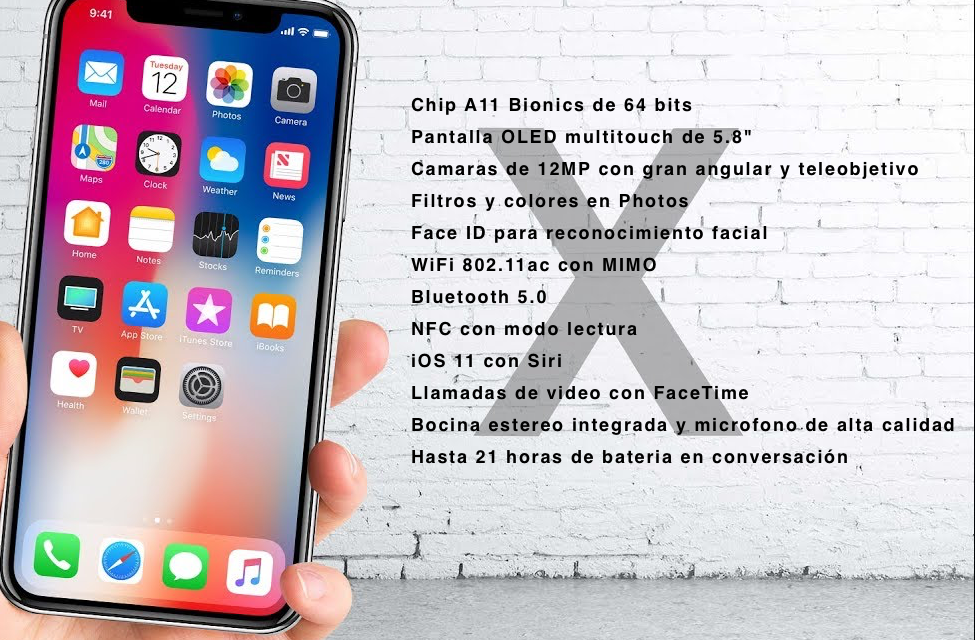
\includegraphics[scale=0.28]{unidades/1_computadoras/1_computadoras/imagenes/iphone_x_specs.png}}

Determine.\\
¿Cuáles de los elementos mencionados corresponden a software?\\
¿Cuáles de los elementos mencionados corresponden a hardware?
\end{exercise}

\begin{exercise}
¿Conoce otros sistemas operativos además de los mencionados? ¿Conoce algo más
sobre los sistemas mencionados?\\
Investigue en internet para descubrir nuevos sistemas y ampliar su conocimiento
de los vistos.
\end{exercise}

\begin{exercise}
¿Se le ocurren otros dispositivos de hardware que use de forma cotidiana?\\
¿Son periféricos de entrada, de salida, de entrada y salida, o de
almacenamiento?
\end{exercise}
